
\begin{figure*}[h]
    \centering
    \begin{minipage}{0.45\textwidth}
        \centering
        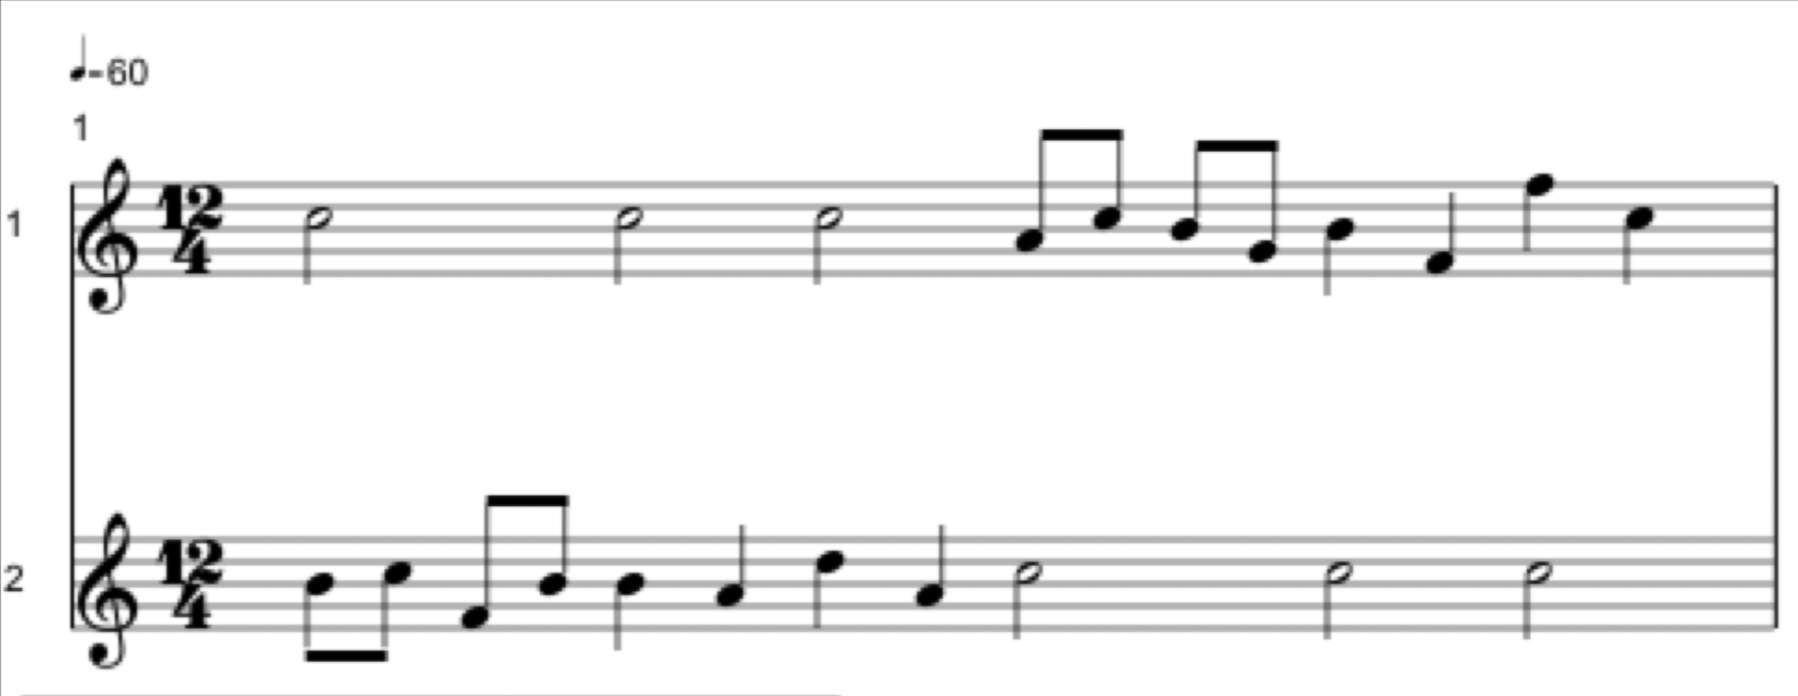
\includegraphics[width=0.9\textwidth]{maxscore-traditional.png} 
                \caption{A score with a random melody rendered in MaxScore’s default layout.
        \label{fig:maxscore-traditional}}
    \end{minipage}\hfill
    \begin{minipage}{0.45\textwidth}
        \centering
        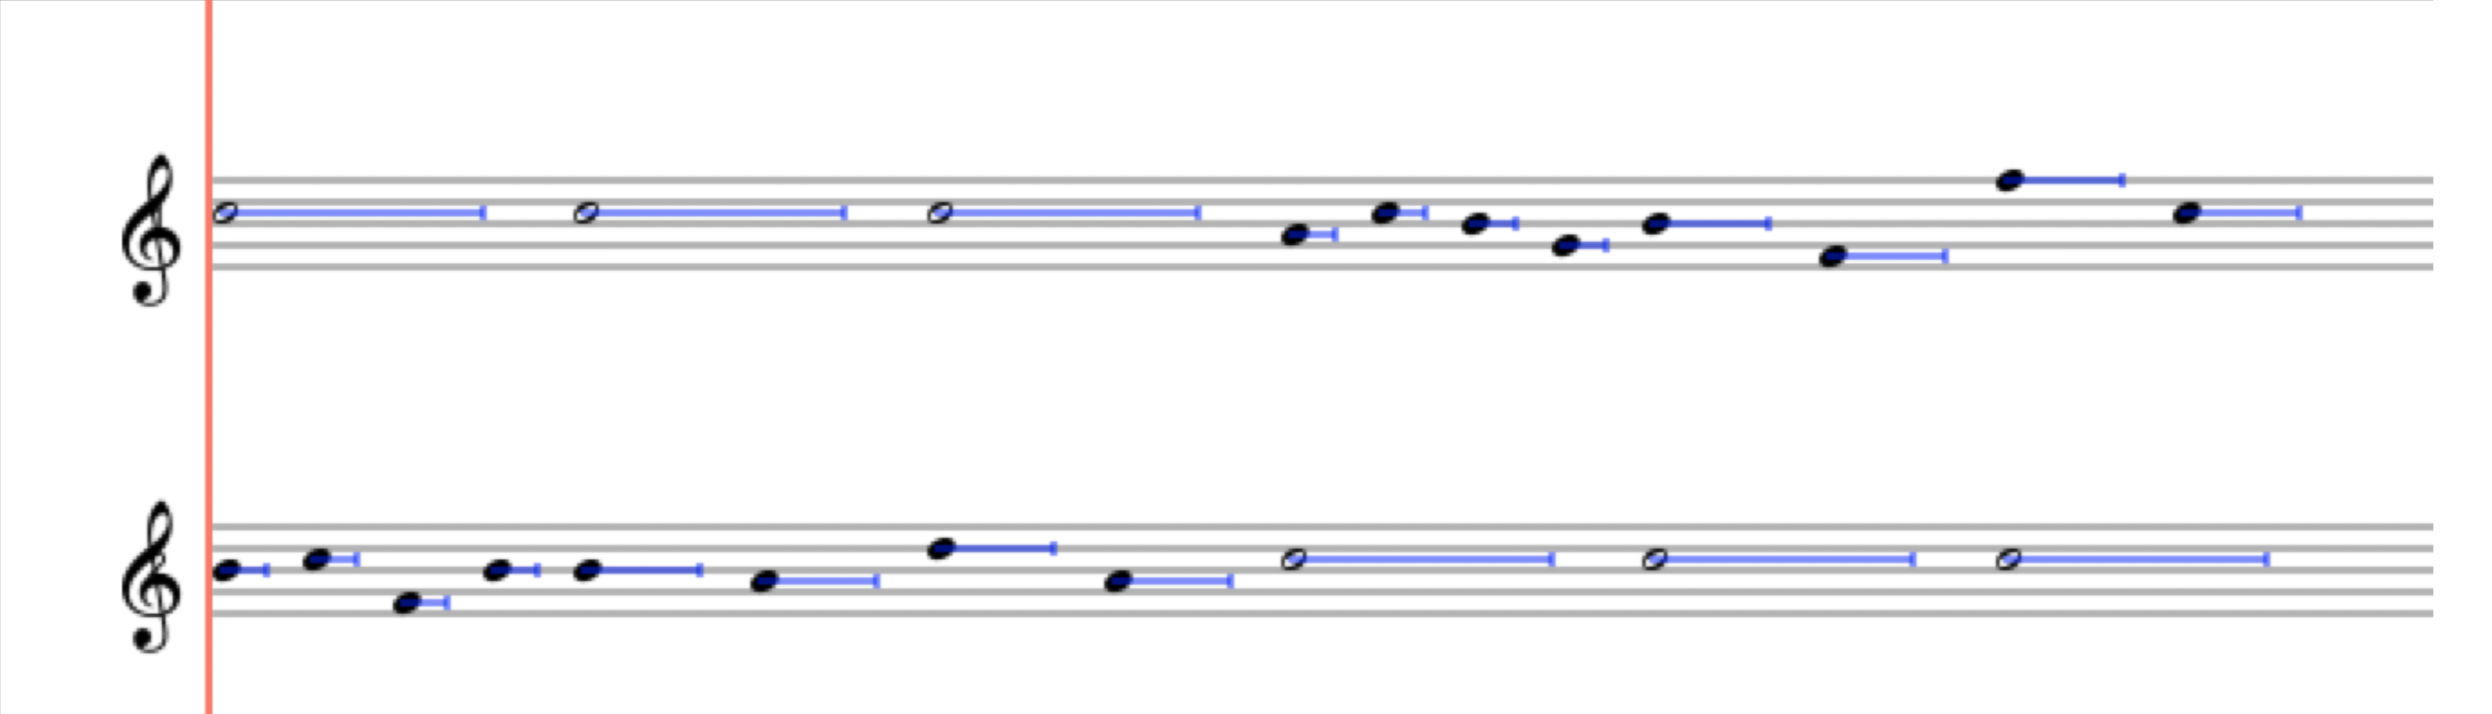
\includegraphics[width=1\textwidth]{maxscore-proportional.png} 
       	\caption{Same score after applying proportional notation. The default hold times indicated by the blue line is set to 80\% of the event’s nominal duration.
\label{fig:maxscore-proportional}}
    \end{minipage}
\end{figure*}

\section{Maxscore}
As mentioned in section~\ref{sec:foundations}., MaxScore possesses a fair amount of flexibility in terms of rendering to a wide array of targets. The JavaScript object render2Browser was created to facilitate the communication between the MaxScore object and hfmt.drawsocket drawing commands. The js object was designed with massive networked music performances in mind. Such performances pose enormous difficulties when distributing large scores with dozens of staves. In performances with Quintet.net, scores containing just a few staves were split into instructions to be reassembled by individual instances of the MaxScore object and rendered locally by the Clients. But doing the same by using a large number of instances in MNMP (which could potentially destabilize the environment and introduce unwanted latency), we resorted to a different strategy by implementing the concept of multi-target rendering, i.e. the MaxScore object renders to any number of browsers instances by routing rendering messages to different destinations depending on the information they carry. Nearly every rendering message contains a set of indexes referring to the notation object it represents (Figure~\ref{fig:maxscore-mesages}). Thanks to those indexes, render2Browser is capable of dynamically reroute a rendering message to a target set by the staffgroups attribute. This attribute can have the following values: score, parts or a list containing either indexes (for individual staves), two indexes joined by hyphens (for a staff range) or any number of indexes joined by plusses (for arbitrary collections of staves) such as in this example: staffgroups 0 1-2 2 0+3.

In addition to splitting and routing messages, the object is also capable of respacing staves so that resulting layout looks acceptable. It does so by querying the MaxScore object during rendering to obtain crucial information about staff spacing and using this information to apply offsets to the y values of each message to be rendered.

\begin{figure}[h]
\centering
\begin{lstlisting}[ mathescape,
						columns=fullflexible,
						basicstyle=\oscfontsize\fontfamily{lmvtt}\selectfont,
						breaklines=true,
						 frame=single ]
tempoqtrequals 20. 21. 0.5 Measure 0. ...
tr 22. 75.959999 0.5 Staff 0. 0. staffnumber1 0. 63. 0.5 Staff 0. 0. timesig4 43. 57. 0.5 Staff 0. 0.
...
StaffLine 0. 0. 4. 0.5 20. 75. 300.660797 75. false
...
frgb 0 0 0
noteheadblack 83.620689 57. 0.5 Note 0. 0. 0. 0.
frgb 0 0 0
no_accidental 75.555557 57. 0.5 Note 0. 0. 0. 0.
frgb 0 0 0
stem 76.620689 79. 0.5 Note 0. 0. 0. 0. STEM_DOWN
RenderMessage staff 0 0 166. 13. 0.5 
rendered Picster-Element[5] 175.3ocUOsnBBCCCzOk6dAg[...]
\end{lstlisting}

\caption{A sample of rendering messages generated by the MaxScore object. 
\label{fig:maxscore-mesages}}
\end{figure}

Figure \ref{fig:maxscore-mesages} shows a sample of rendering messages generated by the MaxScore object. Note that nearly every message is accompanied by indexes referring to the notation object they represent. The RenderMessage message contains a gzip’ed JSON object which in turn codes for a graphical score element such as lines, rectangles, arcs or images.

render2Browser is also capable of animating either any number of cursors moving across a measure/staff or set of measures and staves (see TENOR 2018 paper), jumping over the leading space at the beginning of every measure.

cursor 1 @begin 1 1 @end 2 2 @passes 2 @timestretch 10.

To scroll the entire score another JavaScript object called maxscore.proportionalNotation was created toggling between MaxScore’s default score layout and a proportional representation of it where rests, stems, beams and naturals are hidden and the duration of a note (MaxScore uses the hold time attribute to differentiate between the actual duration of an event and the duration in term of its notated value) is indicated by a line extending from a note. The length of a measure is calculated by obtaining its tempo and time signature values and taking the maxscore.proportionalNotation setTimeUnit attribute into consideration. A durational scaling base value of 0.385 has proven to be optimal for spatially representing the delta time between events. The start message will cause a playhead to appear at the position given by the scoreLeftMargin attribute and instruct the browser to scroll the score. We are planning to also support scores created for the Decibel ScorePlayer in the future.


%describe use of hfmt.drawsocket via Maxscore translation script.




\section{Case study}

Georg's piece in Taiwan


